\documentclass[letterpaper, 10 pt, conference]{ieeeconf}
\usepackage{graphicx}
\overrideIEEEmargins
\usepackage[utf8]{inputenc}
\usepackage[T1]{fontenc}
\usepackage{graphics}
\usepackage{amsmath}
\usepackage{amssymb}
\usepackage{booktabs}

\title{\LARGE \bf
Clasificación Multiclase de Tumores Cerebrales mediante Redes Neuronales Convolucionales con Normalización Empírica
}

\author{Andres Javier RAMBAL VECINO}

\begin{document}

\maketitle
\thispagestyle{empty}
\pagestyle{empty}

\begin{abstract}
El diagnóstico temprano de tumores cerebrales mediante resonancia magnética (MRI) es un desafío crítico en oncología. Este trabajo presenta el diseño e implementación de una Red Neuronal Convolucional (CNN) optimizada para clasificar MRI en cuatro categorías: Glioma, Meningioma, Tumor Pituitario y Tejido Sano. Utilizando un dataset de 7,023 imágenes y una estrategia de normalización basada en estadísticas locales del dominio médico, el modelo alcanzó una exactitud del 88\%. Se analiza la robustez de la arquitectura frente al desbalance de clases y la ambigüedad visual entre tipos tumorales.
\end{abstract}

\section{Introducción}
La detección de neoplasias en el sistema nervioso central requiere una precisión extrema, ya que el margen de error clínico impacta directamente en el pronóstico del paciente. Los tumores como el Glioma y el Meningioma presentan texturas y densidades similares en las imágenes de Resonancia Magnética (MRI), lo que genera variabilidad en los diagnósticos manuales.

Con la evolución de la Visión por Computadora, las Redes Neuronales Convolucionales (CNN) han surgido como el estándar de oro para el análisis de imágenes médicas debido a su capacidad para aprender representaciones espaciales jerárquicas \cite{c1}. A diferencia de los métodos tradicionales, las CNN pueden identificar patrones microscópicos en los píxeles que son imperceptibles para el ojo humano. Este proyecto implementa una arquitectura personalizada que prioriza la generalización mediante técnicas de regularización como Dropout y Normalización por Lotes (Batch Normalization), adaptando el pipeline de datos específicamente a la distribución de intensidades de las MRI \cite{c2}.

\section{Metodología}

\subsection{Dataset y División de Datos}
Se utilizó un dataset público compuesto por 7,023 imágenes de MRI cerebrales en formato bidimensional. La distribución de clases se validó mediante un análisis exploratorio de datos (EDA), identificando 1,621 Gliomas, 1,645 Meningiomas, 1,757 Tumores Pituitarios y 2,000 casos de Tejido Sano. Para garantizar una evaluación científica rigurosa, el dataset se dividió en tres subconjuntos independientes: entrenamiento (70\%), validación (15\%) y prueba (15\%).

\subsection{Preprocesamiento y Normalización}
Dada la naturaleza de las imágenes médicas, que presentan un sesgo significativo hacia el negro en el fondo, se rechazó el uso de normalización genérica (ImageNet). En su lugar, se realizó un cálculo empírico de la media ($\mu \approx 0.186$) y desviación estándar ($\sigma \approx 0.182$) de la totalidad del dataset de MRI. Las imágenes fueron redimensionadas a una resolución de 224x224 píxeles. Para mitigar el sobreajuste (overfitting), se aplicó una estrategia de aumentación de datos que incluyó rotaciones aleatorias de hasta 15$^\circ$ y volteos horizontales (flips), forzando a la red a aprender la morfología del tejido en lugar de la posición absoluta de los objetos.

\begin{figure}[h]
    \centering
    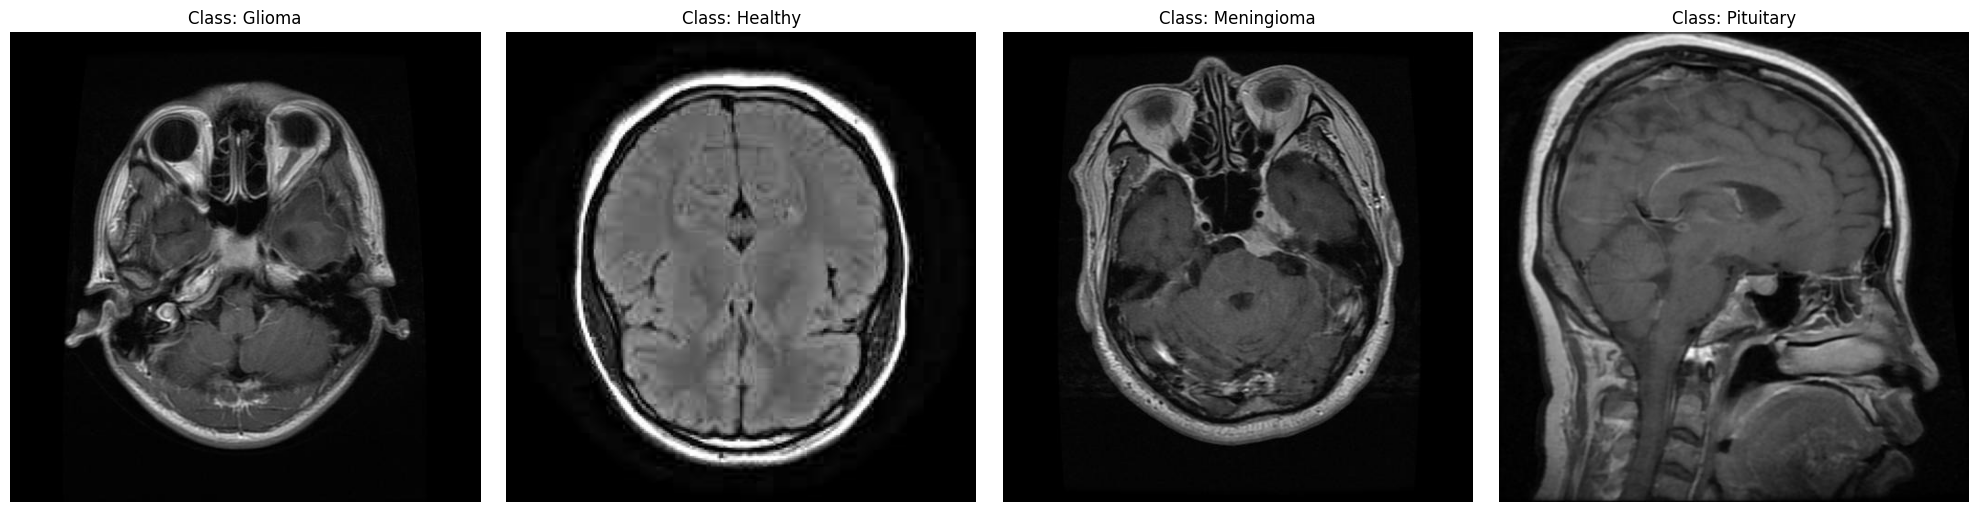
\includegraphics[width=0.9\linewidth]{muestras.png}
    \caption{Visualización de muestras de las categorías Glioma, Meningioma, Pituitaria y Sano (mapeo 'bone').}
\end{figure}

\subsection{Arquitectura del Modelo}
Se diseñó una arquitectura de cuatro bloques convolucionales inspirada en el principio de profundidad progresiva de VGG \cite{c3}. Cada bloque se compone de:
\begin{itemize}
    \item Capa \textbf{Conv2D} con kernels de 3x3 y padding igual para preservar dimensiones.
    \item \textbf{Batch Normalization} para estabilizar la distribución de las activaciones y acelerar la convergencia \cite{c4}.
    \item Activación \textbf{ReLU} para introducir no-linealidad.
    \item \textbf{MaxPooling} de 2x2 para reducir la dimensionalidad espacial.
\end{itemize}

El clasificador final recibe un vector aplanado de 50,176 características, procesado por una capa densa de 512 neuronas con activación ReLU, seguida de una capa de \textbf{Dropout (0.5)} para prevenir la co-adaptación de neuronas \cite{c5}. La salida final utiliza una función \textbf{Softmax} para proyectar las probabilidades sobre las 4 clases médicas.

\section{Resultados}

\subsection{Análisis de Convergencia}
El modelo se entrenó durante 15 épocas utilizando el optimizador \textbf{Adam} con un learning rate de 0.001 \cite{c6}. Como se observa en la Fig. 2, la función de pérdida (\textit{Loss}) presentó un descenso monótono, mientras que la precisión en validación alcanzó la estabilidad rápidamente, indicando un aprendizaje eficiente.

\begin{figure}[h]
    \centering
    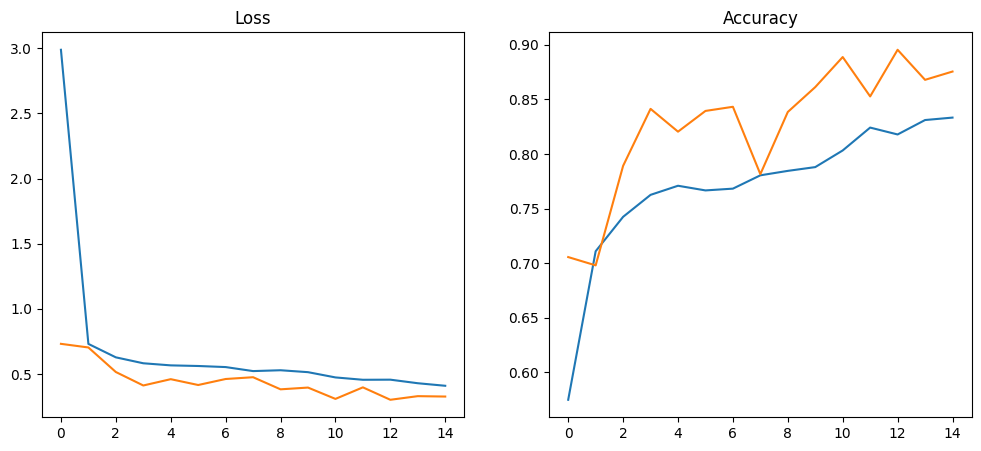
\includegraphics[width=0.95\linewidth]{curvas.png}
    \caption{Curvas de entrenamiento: Precisión y pérdida para los sets de entrenamiento y validación.}
\end{figure}

\subsection{Métricas de Evaluación}
Tras la evaluación en el conjunto de prueba independiente (datos no vistos), el modelo alcanzó una **exactitud global del 88\%**. La red demostró una robustez sobresaliente en la identificación de la clase "Sano" (F1-Score: 0.95), minimizando el riesgo clínico de omitir anomalías. La clase "Tumor Pituitario" obtuvo el recall más alto (0.98), validando que la ubicación anatómica de esta patología es un rasgo altamente discriminatorio para la red.

\section{Discusión}

\subsection{Confusión Meningioma vs. Glioma}
El análisis de la matriz de confusión (Fig. 3) revela que la mayor tasa de error ocurre entre Gliomas y Meningiomas (Recall de 0.68 para el segundo). Desde una perspectiva radiológica, esto se explica por la heterogeneidad visual de estas masas; ambos pueden presentar realce de contraste y bordes irregulares similares en MRI potenciados \cite{c2}. Para resolver esta ambigüedad, futuros trabajos deberían explorar el uso de transferencia de aprendizaje (\textit{Transfer Learning}) con modelos más profundos como ResNet o DenseNet.

\begin{figure}[h]
    \centering
    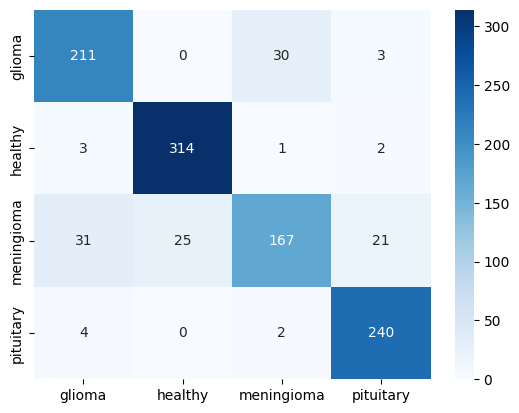
\includegraphics[width=0.8\linewidth]{matriz.png}
    \caption{Matriz de confusión detallando la diferenciación multiclase del modelo final.}
\end{figure}

\subsection{Impacto de la Normalización Empírica}
La decisión de utilizar estadísticas locales fue crítica. Al centrar los datos en la media real de las MRI, se evitó la saturación de gradientes que ocurre al aplicar normalizaciones de imágenes naturales (brillantes y coloridas) a imágenes médicas (oscuras y con alto contraste). Esto permitió que las capas de Batch Normalization mantuvieran el flujo de información durante todo el proceso de entrenamiento.

\section{Conclusiones}
Este estudio valida el uso de CNNs como herramientas de apoyo al diagnóstico oncológico. Con una precisión del 88\% y un alto desempeño en la detección de tejido sano, el modelo propuesto ofrece una base sólida para sistemas de triaje automatizado. La implementación de regularización y preprocesamiento específico de dominio demostró ser la clave para la estabilidad del sistema en problemas de clasificación médica multiclase.

\begin{thebibliography}{99}
\bibitem{c1} Krizhevsky et al., ``ImageNet Classification with Deep CNNs,'' NIPS, 2012.
\bibitem{c2} Cheng et al., ``Enhanced performance of brain tumor classification via region augmentation,'' PLOS ONE, 2015.
\bibitem{c3} Simonyan & Zisserman, ``Very deep convolutional networks for large-scale recognition,'' ICLR, 2014.
\bibitem{c4} Ioffe & Szegedy, ``Batch normalization: Accelerating training by reducing covariate shift,'' ICML, 2015.
\bibitem{c5} Srivastava et al., ``Dropout: A simple way to prevent neural networks from overfitting,'' JMLR, 2014.
\bibitem{c6} Kingma & Ba, ``Adam: A method for stochastic optimization,'' ICLR, 2015.
\end{thebibliography}

\end{document}
